\chapter{Introduction}

\section{Background}


Proper estimation of offshore piles is vital to the life and permanence of the foundation in question. However, due to the uncertainties of soil parameters in the field, the offshore piles are greatly effected. The source of soil uncertainties may come from various reasons, such as  lack of uniformity between in-situ test and laboratory  experiment; spatial variability of soil profile and rationality of the constitutive model, etc. Traditional statistical analysis is based on Monte Carlo, which is time-consuming and laborious. Even if Bayesian theorem provides a possible tool to understand and update the uncertainties for the priors, the amount of the inference analysis is still computationally heavy, thus bring big challenges for the pile design.
One typical soil profile can be shown in \cref{fig:fig1.1}, it can be seen that:

\setlength{\parskip}{0pt}
\setlist[itemize]{itemsep=0pt,topsep=0pt,parsep=0pt,partopsep=0pt}

\begin{itemize}

    \item Fluctuating untrained shear strength curve indicates the spatial  variability
    \item Non-uniformity exists between in-situ test and laboratory experiment

\end{itemize}

\begin{figure}[htbp]
    \centering
    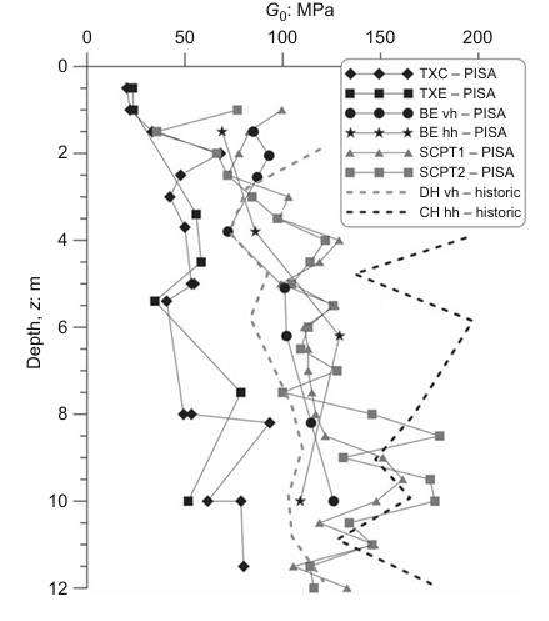
\includegraphics[width = 90mm]{Figures/figure1.pdf}
    \caption{Untrained strength profile at Cowden \protect\cite{zdravkovic2020}}
    \label{fig:fig1.1}
\end{figure}


\section{Challenges}

Bayesian theorem provides a possible tool to understand and update the uncertainties for the priors as shown in \cref{equation 1.1}.
\begin{equation}
P(A|B) = \frac{{P(B|A) \cdot P(A)}}{{P(B)}} \label{equation 1.1}
\end{equation}
$P(A|B)$: posterior: Distribution of soil parameters;$P(B|A)$:likelihood: observed data and FE simulation based on priors; $P(A)$: prior: Soil parameters from lab/field.
The challenges are:

\begin{itemize}
    \item The amount of Inference analysis is time consuming (each soil layer can contain 2 to 14 parameters)
    \item How to get the best possible soil parameters distribution, based on the given priors, while avoiding extreme calculations.

\end{itemize}